\chapter{Introdução}

  A Organização das Nações Unidas (ONU) divulgou em 2015 o seu relatório referente
  às perspectivas de crescimento populacional, que constatou uma população mundial
  de 7,3 bilhões na metade do ano de 2015, projetando ainda, para 2030, um aumento
  para 8,5 bilhões \cite{ONU2015}. Esse aumento populacional representa também um
  aumento significativo na demanda por alimentos, energia e infraestrutura.
  A indústria agrícola tem um papel essencial ao satisfazer essa demanda por alimentos,
  de forma que o aumento de produtividade e eficiência é muito importante.
 
  A utilização de tecnologias para o aperfeiçoamento do processo produtivo e
  diminuição de custos já é há muito conhecida. Segundo \cite{RAMIZ1988},
  “os custos de produção podem variar por diversos motivos. Pode-se destacar a
  utilização intensiva ou não de tecnologia”. Uma das soluções propostas é a
  utilização de robôs automatizados (também conhecidos como rovers) para a
  análise do solo e de suas propriedades e necessidades, tornando customizado
  o uso de insumos para o processo produtivo.

  Estas tecnologias também podem melhorar os números em termos de sustentabilidade.
  O setor agrícola é o que mais consome e também o que mais desperdiça água doce no país.
  Aproximadamente 70\% da água utilizada no Brasil é destinada as suas atividades
  e quase metade desse valor é jogada fora. Entre os motivos do desperdício estão
  irrigações mal executadas e falta de controle do agricultor na quantidade usada
  em lavouras e no processamento dos produtos \cite{fao2013}.
    
  \section{Problemática}
  
  O desenvolvimento da agricultura através de métodos tradicionais vem se
  mostrando cada dia mais obsoleto, uma vez que não acompanha inovações
  tecnológicas \cite{ROCHA2015}. Essa transferência de tecnologia para aplicações
  práticas em processos produtivos muitas vezes ocorre de forma lenta, já que
  os produtores se mostram resistentes a alterações em um sistema que funciona
  relativamente bem. Entretanto, a não adoção dessas tecnologias acarreta
  prejuízos das mais diversas formas. Ao abdicar de uma análise detalhada do
  solo, um produtor agrícola gera custos desnecessários de irrigação, nutrição
  do solo, controle de acidez, além da inevitável queda na qualidade do produto
  final. Mesmo que exista uma análise laboratorial por amostragem, esse método
  não demonstra ser tão eficiente quanto uma análise automatizada, já que essa
  análise somente é feita em laboratórios específicos, podendo a amostra,
  durante o seu transporte, ter alterações em suas características, o que pode
  prejudicar o resultado final da análise. Uma produção baseada em inovações
  tecnológicas garante, portanto, o aumento de produtividade, diminuição de
  custos e reduz significativamente possíveis falhas humanas no diagnóstico de
  problemas.

  Para uma descrição mais clara e formal do problema, foi utiliza o seguinte
  framework de descrição de problema:

  \textbf{O problema:} Falta de monitoramento da umidade nas dimensões espaço/tempo
  para decisões de apoio à produção.

  \textbf{Afeta:} Produtores de morangos. 

  \textbf{Cujo impacto é:} Má irrigação das plantações, diminuição da qualidade
  do produto final e desperdício de água.

  \textbf{Uma solução bem sucedida seria:} A criação de um robô que automatiza
  a coleta da umidade em diversos pontos de uma lavoura.

  As causas para o problema, junto ao problema, foram representadas em um diagrama
  de causa e efeito, também conhecido como fishbone, conforme é possível ver
  na figura abaixo.

  \begin{figure}[h]
    \centering
    \label{fig01}
      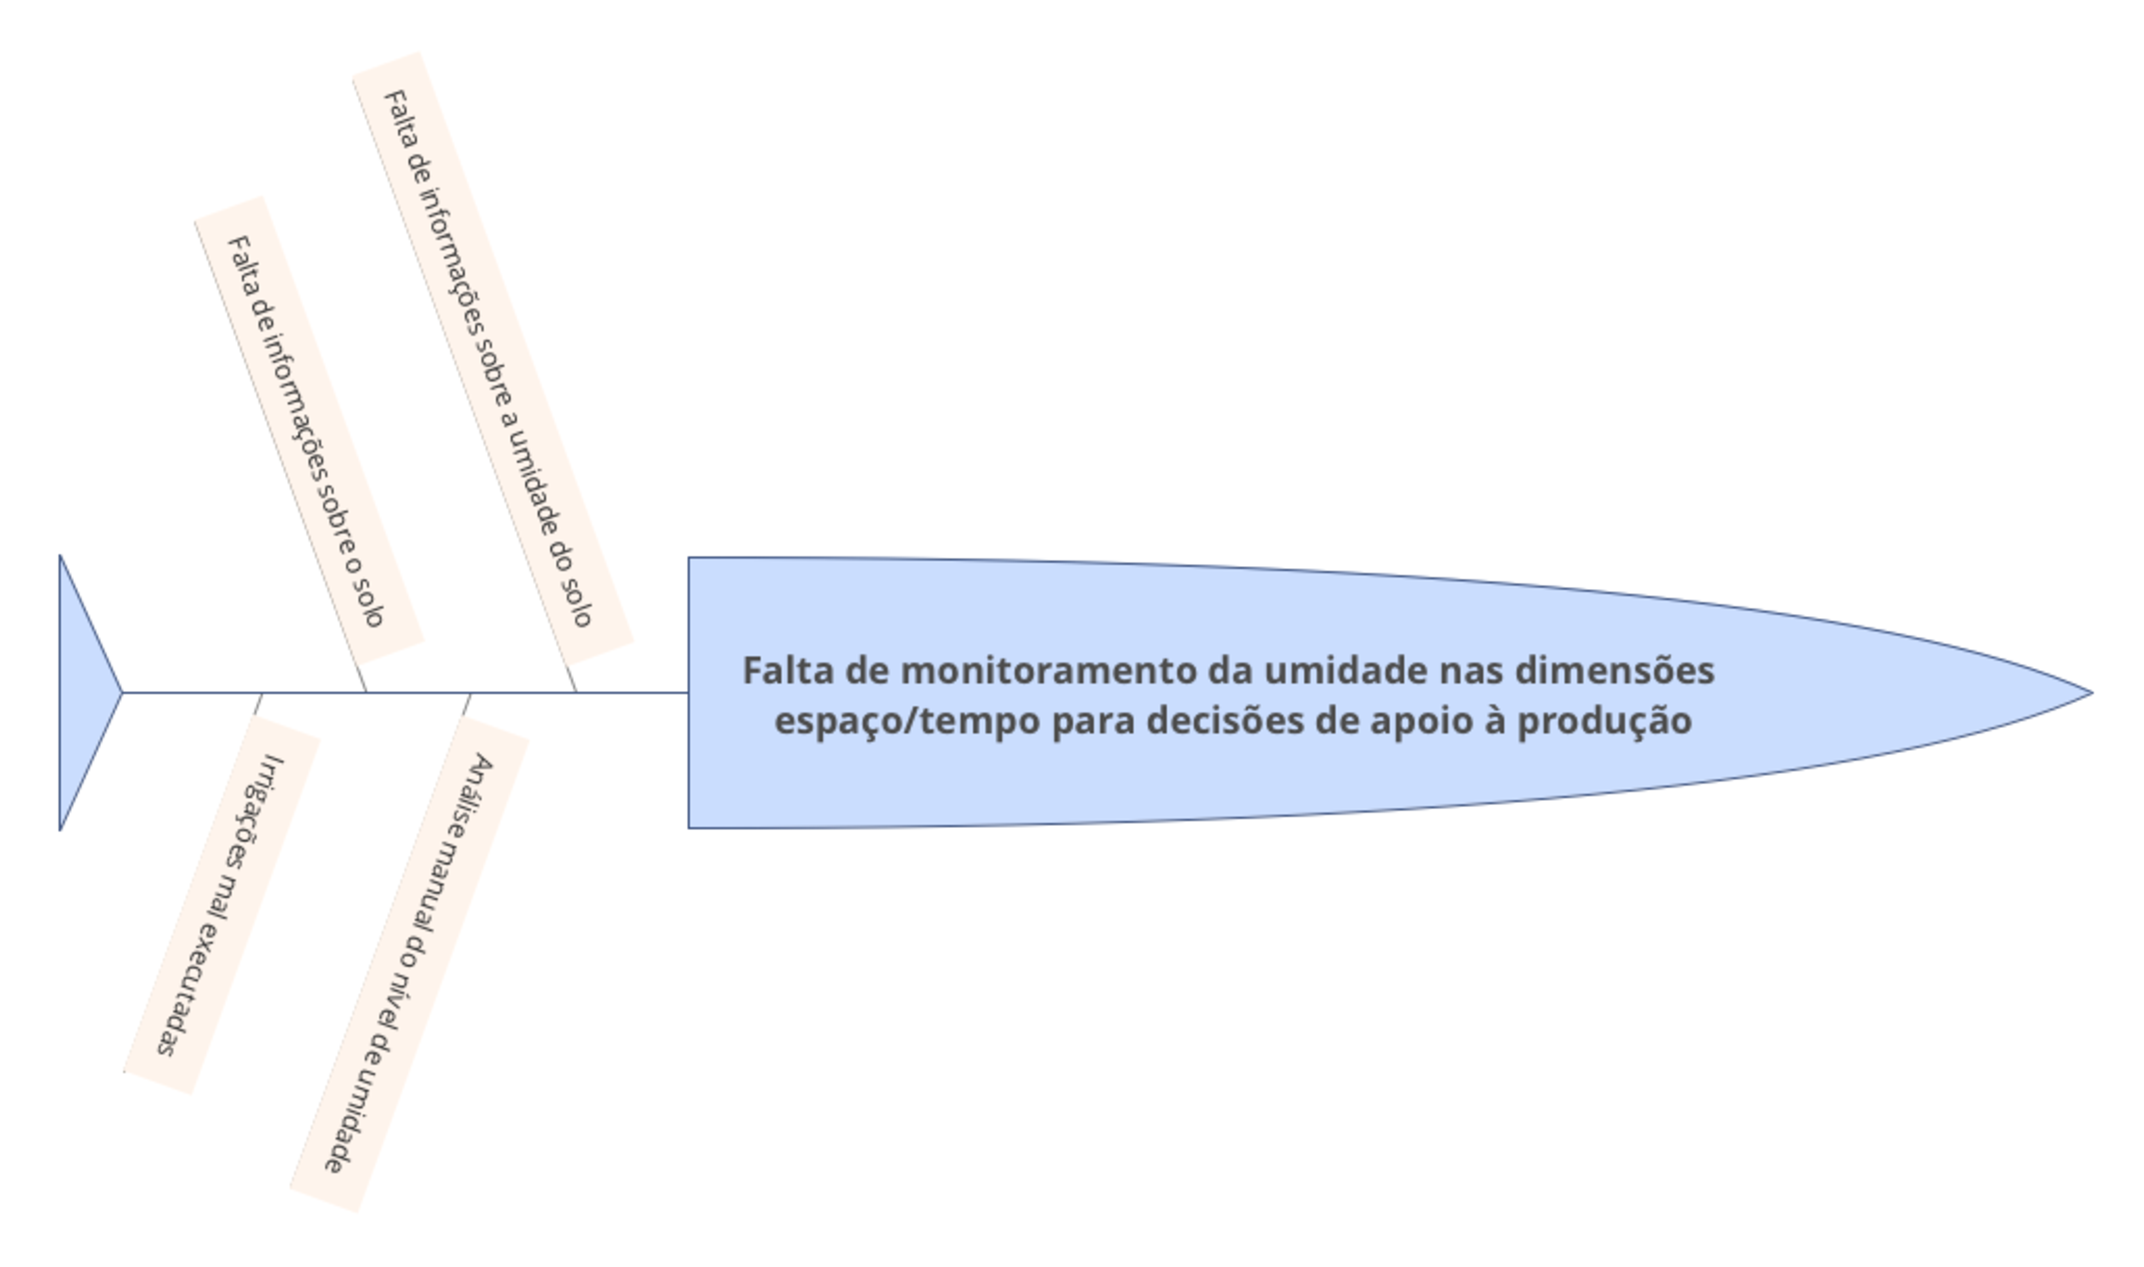
\includegraphics[keepaspectratio=true,scale=0.5]{figuras/fig01.eps}
    \caption{Diagrama de Fishbone para mapeamento do problema}
  \end{figure}

  \section{Estado da Arte}

  Dentre as tecnologias existentes, protótipos como o rover, desenvolvido pela
  Embrapa em conjunto com a Universidade de São Paulo, e o “Robô Autônomo para
  Monitoramento do Solo” pela Universidade de Virgínia, se destacam como
  potenciais tecnologias no ramo da automatização agrícola e possuem grande
  potencial de inserção no mercado.  Entretanto estas tecnologias não são
  amplamente utilizadas no mercado por se tratarem de protótipos e não haver
  produção em massa consolidada.

  O rover desenvolvido pela EMBRAPA utiliza uma tecnologia de análise óptica
  para adquirir dados do solo. Essa tecnlogia se chama LIBS (Espectroscopia de
  emissão óptica com plasma induzido por laser), onde um laser de alta energia
  é focalizado sobre o solo, fazendo com que seja formado um plasma.
  Esse plasma realiza uma análise multielementar do solo, \cite{ARCHILA2014}.

  \begin{figure}[h]
    \centering
    \label{fig01}
      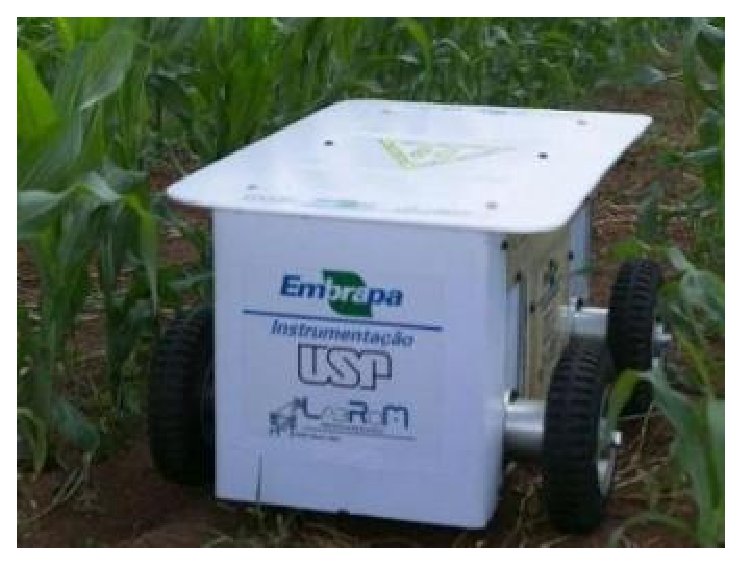
\includegraphics[keepaspectratio=true,scale=0.5]{figuras/fig02.eps}
    \caption{Rover desenvolvido pela EMPRAPA com tecnologia LIBS. Fonte: \cite{ARCHILA2014}}
  \end{figure}

  \section{Justificativa}

  \section{Objetivos}
  \subsection{Geral}
  \subsection{Específicos}

  \section{Escopo}
